% !Mode:: "TeX:UTF-8"

\chapter{实验环境}

\section{Gym和Pyrobolearn}\label{introenv}
Gym\cite{brockman2016openai}是一个由OpenAI团队开源的强化学习仿真环境,它已经成为了评价最先进的基线强化学习算法或机器人控制算法的标准环境。
Mujoco\cite{todorov2012mujoco}是一个著名的商业物理仿真引擎,它在强化学习和机器人学中得到广泛应用,并成为Gym中机器人相关的环境的默认仿真引擎。
在接下来的几章中,Gym将被用来验证算法正确性,或被用于更方便地与其他现有算法进行对比。

Gym提供一个Python语言的接口并且已经被包含在了Python包检索中。
Gym需要使用OpenGL的开源库GLFW来进行渲染。
它可以直接使用Python包管理器\emph{pip}进行安装。
在Gym中,有很多内置的环境,包含大量著名的和强化学习有关基本任务可用于验证强化学习算法,并提供了统一的接口。
例如,它包含一个经典的名为“推车杆”的控制任务,这个任务要求智能体通过水平地移动推车来平衡一个底部用自由活动的关节连接到推车上的杆。
一个正常的强化学习算法应当可以在较长时间内避免杆失去平衡并倒下。

Mujoco(Multi-Joint dynamics with Cotact)是一个致力于仿真复杂关节运动、碰撞和多物体接触的物理引擎。
它集成了粒子系统仿真、约束求解器、有限元积分器和凸优化器等等工具。
它使用ANSI C编写并有一个Python的API封装。
在Gym中,\emph{FetchReach-v1}环境需要使用Mujoco作为仿真器,因此在实验中Mujoco、OpenGL和Gym等工具都被安装在Ubuntu 20.04系统中,并设置了环境变量以保证正确的动态链接库\emph{libGL.so}和Mujoco的二进制分发被加载。

一个\emph{FetchReach-v1}环境的截图展示在图\ref{fetchreach-v1}中。
    \begin{figure}
        \centering
        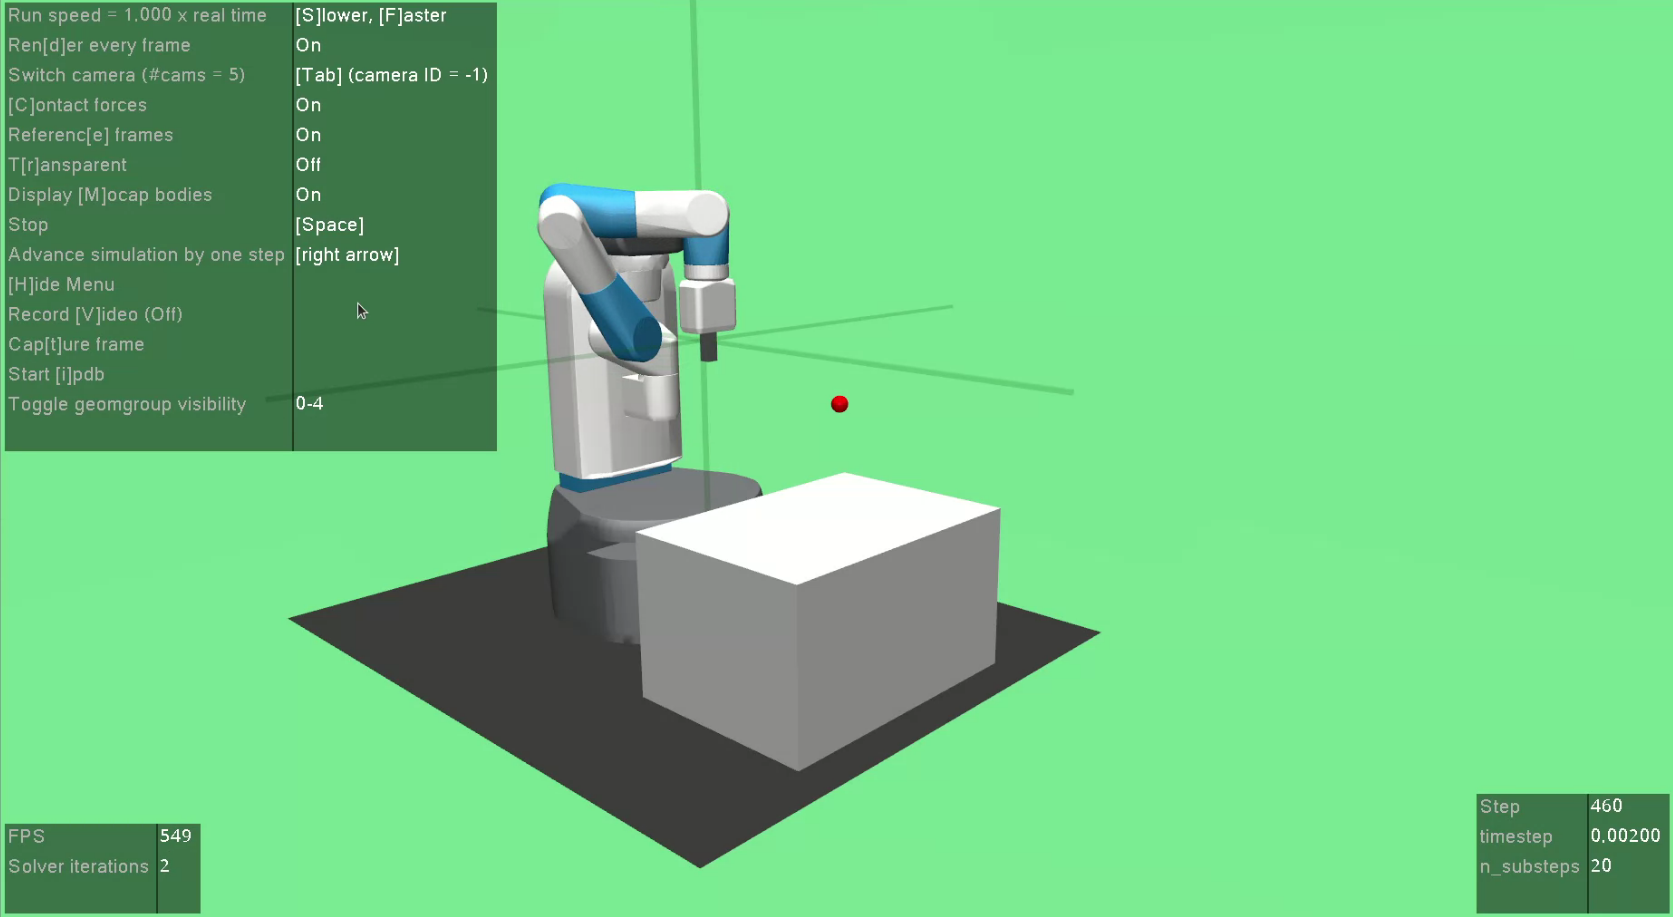
\includegraphics[width=0.5\textwidth]{fetchreach-v1.png}
        \caption{FetchReach-v1环境的截图}
        \label{fetchreach-v1}
    \end{figure}
其中有一个机械臂被放在一张桌子前。
在每个片段刚开始时,这个机械臂的状态都会被重置,而一个红点则会随机地出现在桌子上方的某处。
机械臂智能体需要在片段的限制时间内使自己的末端执行器到达这个红点附近来完成任务并获得奖励。
在片段的每一个时间步中,都会有观测值提供给此机械臂智能体。
观测值包括指示关节状态、末端执行器位置坐标信息作为已完成的目标,和红点的位置坐标信息作为期望目标。
指示关节状态的观测值$o\in \mathbb R^{10}$是一个10维的向量,而末端执行器的坐标$g^a \in \mathbb R^3$和红点的位置坐标$g^d\in\mathbb R^3$都是3维的向量。
因此提供给机械臂智能体的状态向量是一个16维的向量$s=(o, g^a, g^d)\in \mathbb R^{16}$。
如果末端执行器和红点之间的距离小于一个阈值,一个值为0.0的奖励会被提供给机械臂智能体,否则一个值为-1.0的奖励会被提供给它。
机械臂可以采取的动作是一个4维的取值在-1到1之间的向量,即$a\in[-1,1]^4$。

\section{Pyrobolearn和Pybullet}
虽然使用Gym和Mujoco的功能已经可以覆盖本课题的大部分实验,但是由于Mujoco是商业仿真软件,且可定制性不强,因此有必要使用开源的替代品,即Pyrobolearn和Pybullet,来设计本课题中的主体实验。

Pyrobolearn是一个专门设计来训练智能机器人的框架\cite{delhaisse2019pyrobolearn}。
它目前仍然在开发中,但是大部分实验中用到的功能已经足够稳定。
一些尚未在其中实现的功能也可以通过继承现有类来进行自定义。
与Gym相似,Pyrobolearn也有一个默认的物理引擎。
这个物理引擎叫做Pybullet\cite{coumans2016pybullet}。
它是一个C++编写的开源的物理引擎Bullet3在Python接口的封装,并可以提供本文中需要的所有仿真功能。它可以实时地检测碰撞,并可以精确地仿真多物理现象,这保证了它可以被用于本文需要的机器人和物体交互仿真的研究需求。
虽然Pyrobolearn也有一个使用Mujoco作为仿真器的接口,但是它对Mujoco的支持尚未稳定,因此本文的实验选择了使用Pybullet作为仿真器。

使用Pybullet作为仿真器,Pyrobolearn可以被用来仿真多种经典的机器人控制和强化学习问题。
实际使用中,一个物理世界对象包含了一些固定的物理量,例如重力方向和摩擦系数,并可以加载物体和机器人。
一个世界对象在构造过程中通常要提供一个仿真器,本文提供了Pybullet作为仿真器。
在世界对象构造完成后一个由仿真器生成的世界相机会被提供给世界对象作为一个属性。

在接下来的使用Pyrobolearn的实验中,全部都使用了\emph{Basic World}类型的世界对象,其中重力加速度向量为笛卡尔坐标系中的(0.0, 0.0, -9.81),横向摩擦系数为1.0,旋转摩擦系数为0.0,滚动摩擦系数为0.0,线性阻尼为0.04,角阻尼为0.04。

渲染后的世界相机下的\emph{Basic World}世界如图\ref{basicworld}所示。
    \begin{figure}
        \centering
        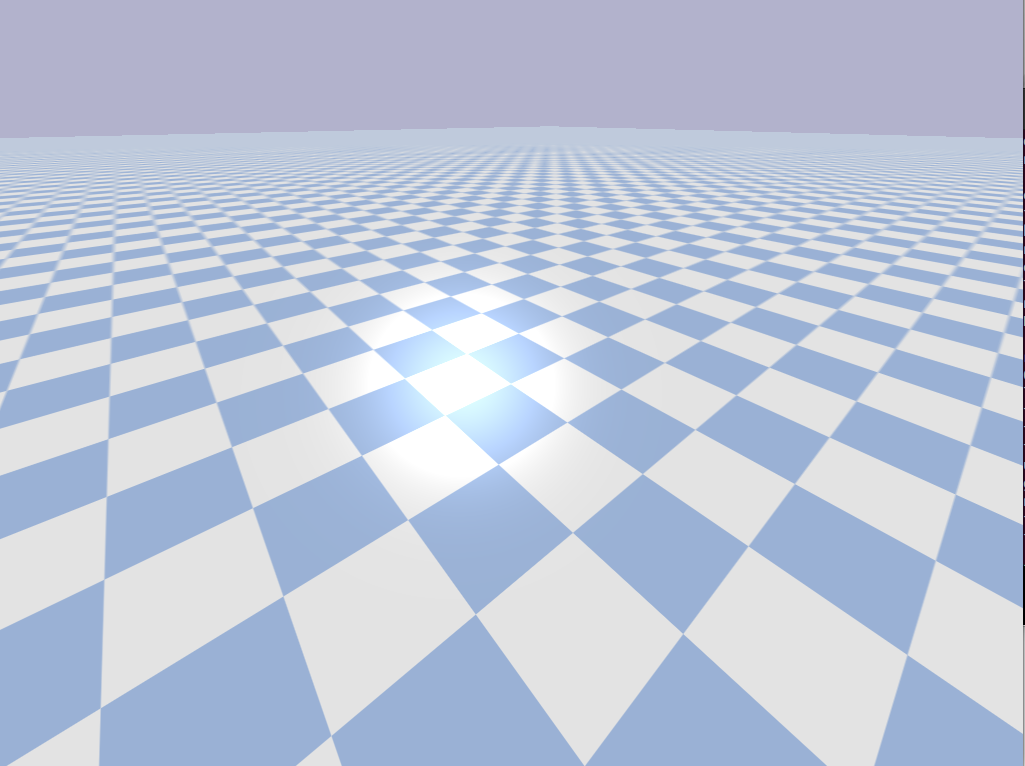
\includegraphics[width=0.3\textwidth]{basicworld.png}
        \caption{空白的\emph{Basic World}世界渲染结果}
        \label{basicworld}
    \end{figure}
默认情况下,没有物体和机器人被加载,只有地面和基本物理量被初始化。

两种不同的机械臂分别在初步实验和主体实验中使用。其中一个来自于Gym环境,另一个来自于Pyrobolearn框架。

在基于Mujoco的几个Gym环境中,一个和Fetch研究平台中的Fetch便携机械臂具有相同参数的机械臂被用作默认的唯一一个与环境交互的机器人\cite{Wise2016FetchF}。
Fetch便携机械臂有7个自由度。
在本文中使用到的\emph{FetchReach-v1}环境中,只有其中的4个被使用。
如第1节所述,\emph{FetchReach-v1}环境中的状态向量由Fetch机械臂的关节的位置信息、末端执行器的笛卡尔坐标和红点的笛卡尔坐标构成。

Pyrobolearn框架中的主体实验使用了一个叫做WAM的机械臂。
WAM机械臂可以配备手指终端执行器,它们一共有15个自由度,这意味着动作空间是非常高维的。
在\emph{Basic World}世界中加载的WAM机器人如图\ref{wam}所示。
    \begin{figure}
        \centering
        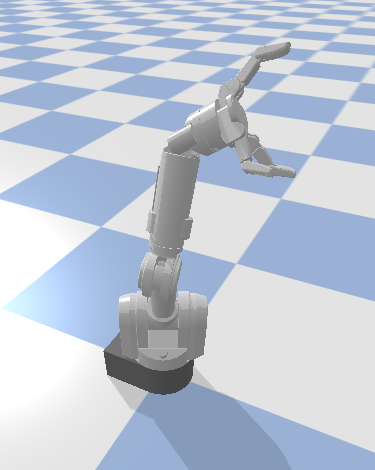
\includegraphics[width=0.3\textwidth]{wam.png}
        \caption{\emph{Basic World}中的WAM机器人渲染结果}
        \label{wam}
    \end{figure}

\section{实验框架}\label{expframe}
本文中所有的实验都有可更改目标的状态,这意味着智能体可以获知当前已完成的目标和期望的目标。
假设期望的目标用一个3维的笛卡尔坐标表示,已完成的目标用机器人的末端执行器的笛卡尔坐标表示。
通常情况下,当这两个坐标间的距离小于一个阈值时,表示任务已经顺利完成。

形式化地,一个状态向量$s\in\mathcal S$是一个由3个向量构成向量,即$s=(o,g^a,g^d)$,其中$o$是观测到的环境中的物理量构成的向量,$g^a$是已完成的目标,$g^d$是期望的目标。
一个环境奖励函数$reward:\mathcal S\to \mathbb R$是由环境反馈决定的智能体在交互中可获得的奖励。

在实验中,因为目标可以方便地修改,所以可以使用事后经验重放算法,这也使得定义具有稀疏奖励的开放任务,并在其中使用多种方法训练高探索效率和泛化能力的智能体成为可能。

智能体与环境的交互在实验中被组织为分离的片段。
每个片段都有相同的最大时间步数$T$。
智能体应当在最大时间步数的限制$t\leq T$下完成一个特定的开放任务并获得较高的奖励。
对于\emph{FetchReach-v1}环境,最大的时间步数为50.
对于在Pyrobolearn框架下的主体实验中自定义的环境中,最大的时间步数为100或200.
智能体可以把在交互中获得的迁移信息$(s_t,a_t,r_t,s_{t+1})$保存在重放缓存中以便之后采样和训练。

对每个片段,最后一个时间步的下一个状态$s_{T+1}$不应被用于训练,因为当环境处理这个状态时这个片段已经结束,因此它不会导致未来的任何奖励。
为了防止在训练过程中使用这个状态,可以引入一个掩膜变量$m$,并与根据$s_{t+1}$计算得出的动作价值函数值相乘。
当$t<T$时,令$m=1$,当达到最后一个时间步,即$t=T$时,令$m=0$,并将$m$和迁移信息一同放入重放缓存中以便训练时与上述动作价值函数相乘。

在每个实验的片段开始时都引入了随机初始化。

对于\emph{FetchReach-v1}环境中的实验,在片段的第一个时间步之前,Fetch便携机械臂的关节位置被初始化为一个固定的起始位置,由红点表示的期望目标则随机地初始化为桌面上的一个位置。

在自定义的Pyrobolearn环境中,在片段开始之前,WAM机械臂上的关节位置被随机初始化,期望的目标也被随机地初始化在1米以内,其中目标的$z$坐标被初始化为0.5,$x,y$则从$[-1,1]$的均匀随机分布中采样。
与\emph{FetchReach-v1}环境中相比,自定义的环境中机械臂的初始状态是随机的,这会给此开放任务带来更多的复杂性。
有时候WAM机械臂的随机初始状态距离目标非常远,这会导致任务理论上不可能完成。

\section{Gym初步实验系统设计}\label{gymexp}

Gym环境下的实验程序按照类图\ref{gymuml}所示的方式组织。
    \begin{figure}
        \centering
        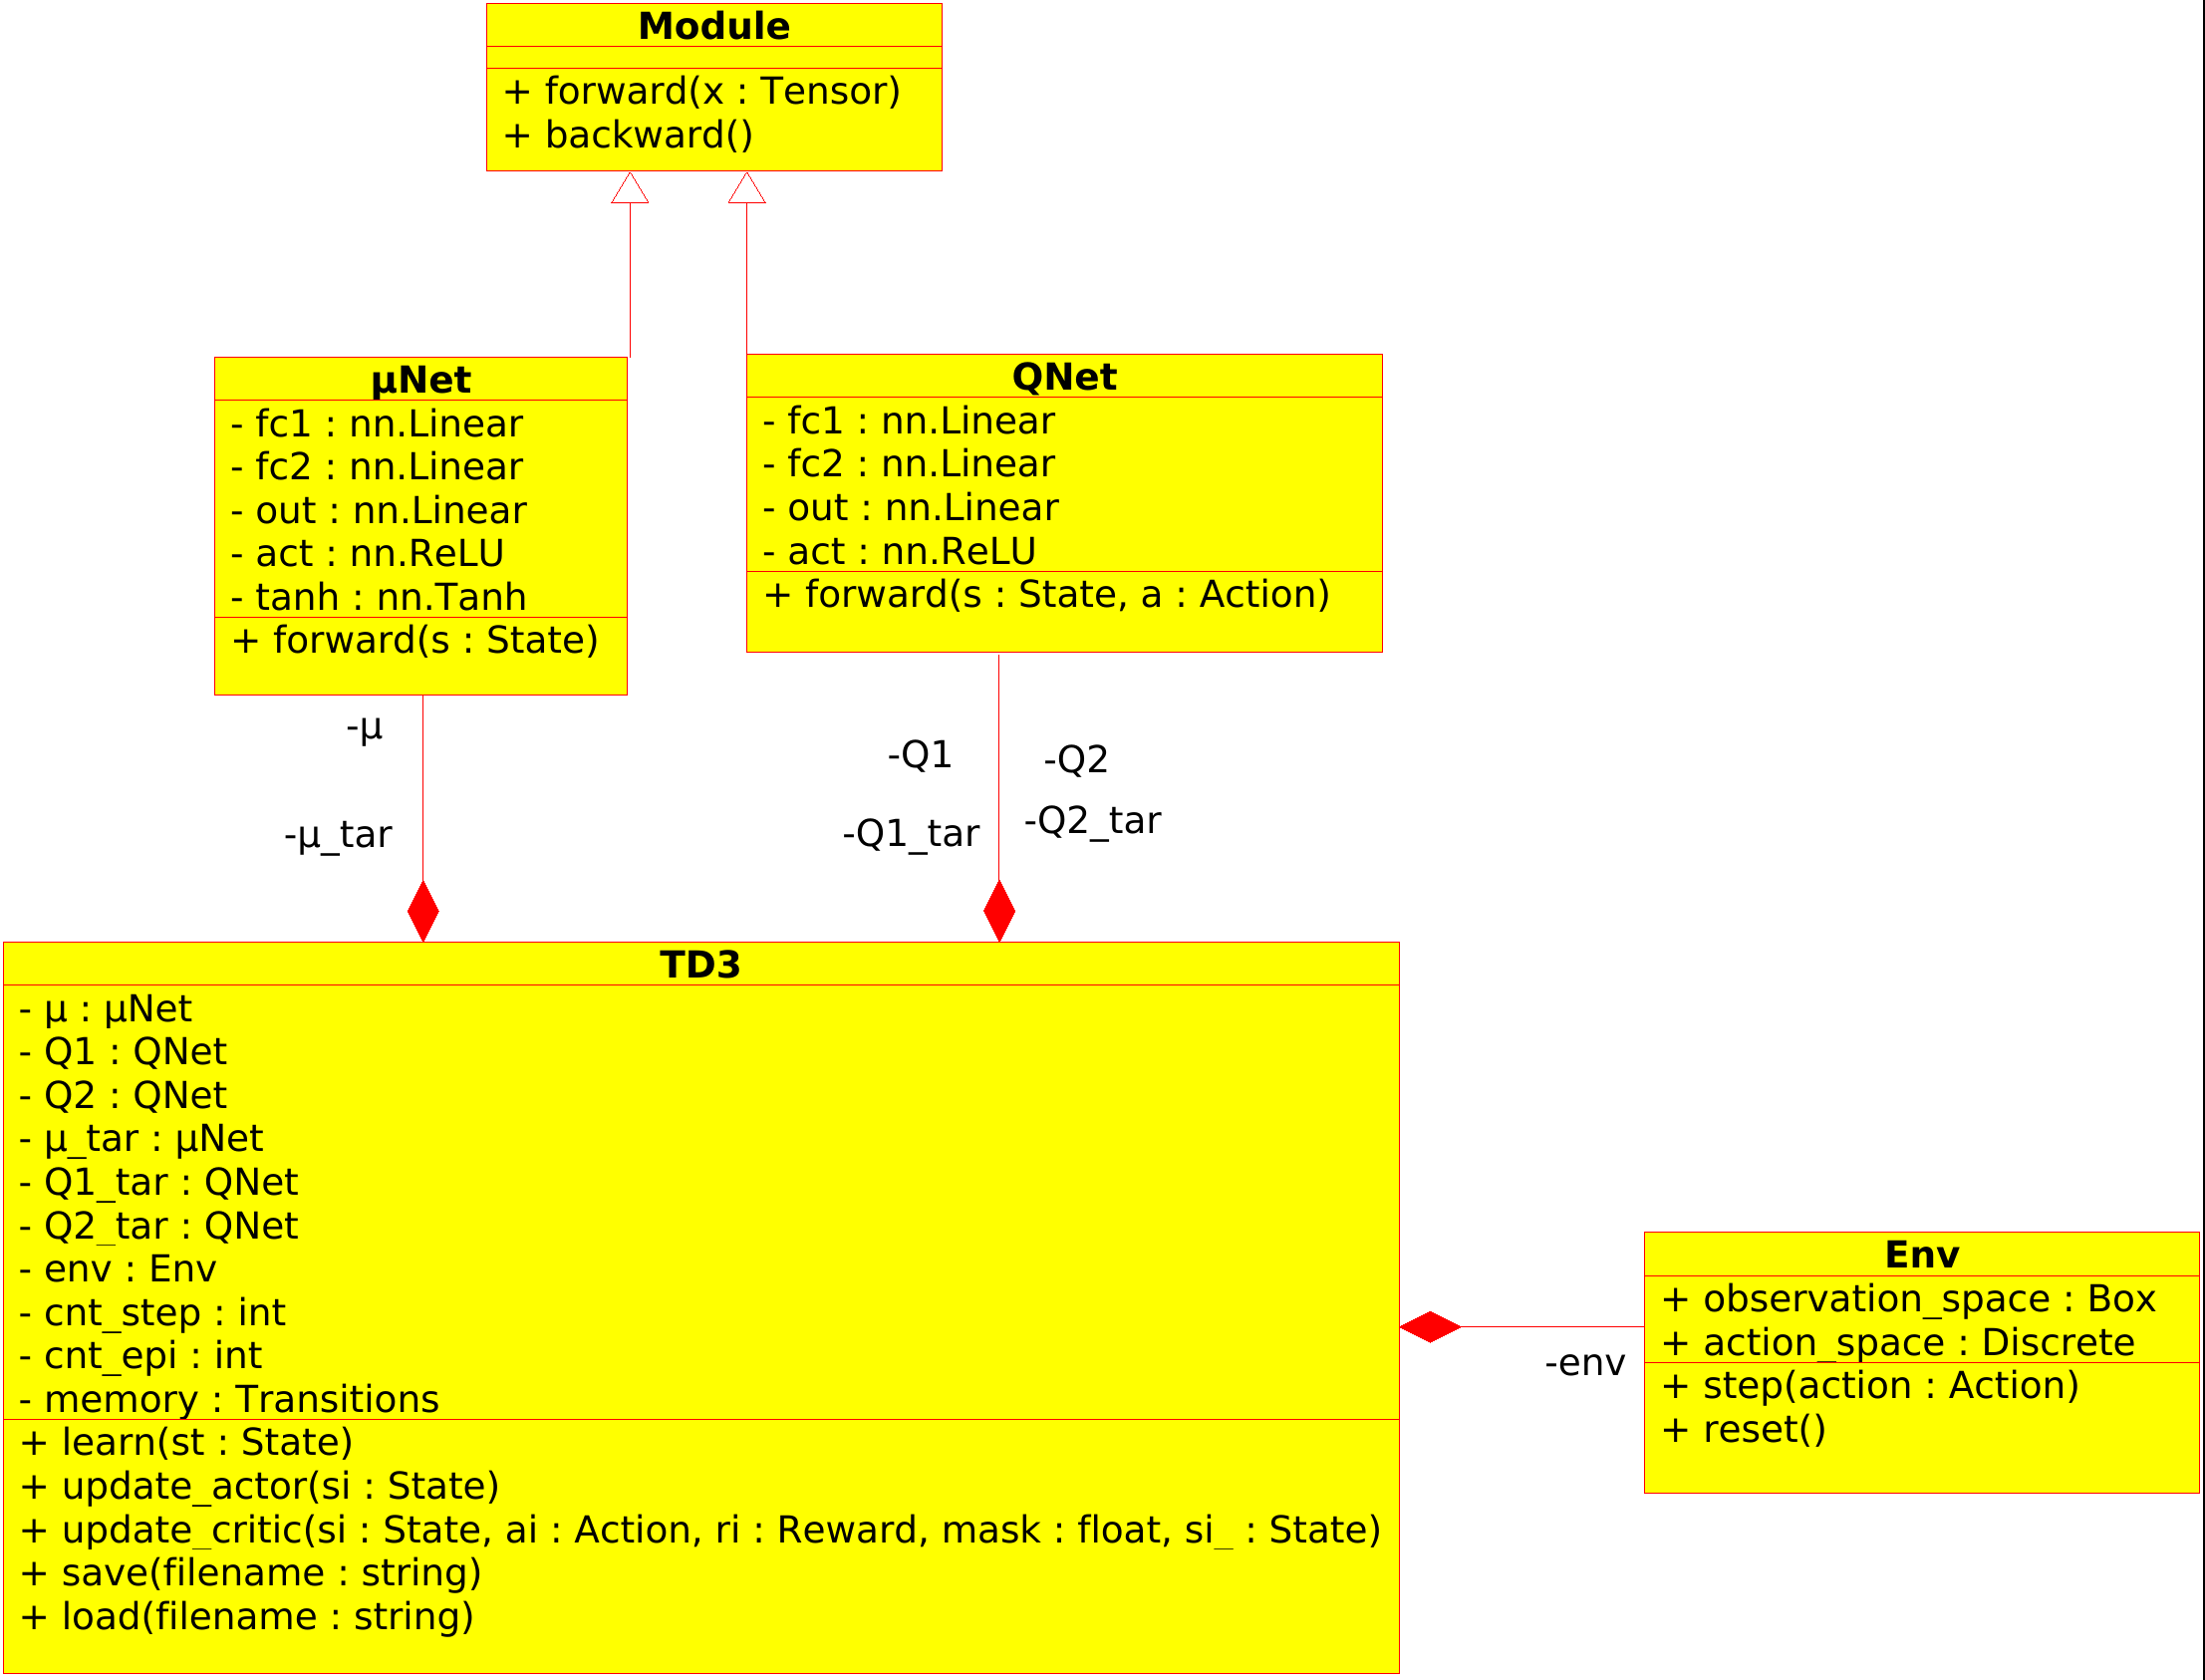
\includegraphics[width=0.6\textwidth]{gymuml.png}
        \caption{Gym初步实验程序类图}
        \label{gymuml}
    \end{figure}
其中Module是Pytorch中的神经网络模块,μNet和QNet通过继承自动获得反向传播的方法backward。
$\mu$,Q1和Q2分别是演员网络,评论家网络1和评论家网络2;$\mu$\_tar,Q1\_tar和Q2\_tar分别是对应的靶网络。
每调用一次TD3对象的learn方法,都会进行一个时间步的仿真,时间步计数器cnt\_step和片断计数器cnt\_epi相当地进行自增运算,并把生成的迁移$(s_t,a_t,r_t,mask_t,s_{t+1})$存入重放缓冲memory中。

上述仿真过程是通过调用环境对象env的step方法来实现的,step方法接收根据演员网络在接收当前状态$s_t$后输出的动作结合相应随机策略生成的动作$a_t$,进行一个时间步的仿真,并输出下一个状态$s_{t+1}$,奖励值$r_t$,此片断是否已经结束$done$和其他信息。
在\ref{expframe}中所述的掩膜$m$可以与折扣系数$\gamma$合并,根据如下公式计算新的掩膜:
\[
m=\begin{cases}
          0, & \text{若} done=True \\
          \gamma, & \text{其他}
\end{cases}
\]

当cnt\_step和cnt\_epi满足一定条件时,update\_actor方法或update\_critic方法会被触发。
在update\_actor和update\_critic方法中,首先对重放缓冲memory进行采样,采样后对采集到的批次迁移数据根据\ref{HERsec}中描述的过程进行事后经验重放。
最后使用如下损失函数计算梯度并用反向传播更新网络权重:
\begin{align}
    & L_\mu = -\sum_i^N\frac{Q_1(s_i, \mu(s_i))}{N} \\
    & L_{Q_1} = \sum_i^N\frac{r_i + m \min\{Q_1'(s_{i+1},\mu(s_{i+1})), Q_2'(s_{i+1},\mu(s_{i+1}))\} - Q_1(s_i,a_i)}{N}\\
    & L_{Q_2} = \sum_i^N\frac{r_i + m \min\{Q_1'(s_{i+1},\mu(s_{i+1})), Q_2'(s_{i+1},\mu(s_{i+1}))\} - Q_2(s_i,a_i)}{N}
\end{align}
其中$\mu, Q_1, Q_2, \mu', Q_1',Q_2'$ 分别对应前述$\mu$,Q1,Q2,$\mu$\_tar,Q1\_tar和Q2\_tar。
为保证实验结果可复现,在经过多次迭代之后要使用save方法保存网络权重,并在测试时使用load方法加载。

上述Q1网络,Q2网络,Q1\_tar网络和Q2\_tar网络都具有相同的网络结构,它们的网络结构如图\ref{gymQnet}所示。

    \begin{figure}
        \centering
        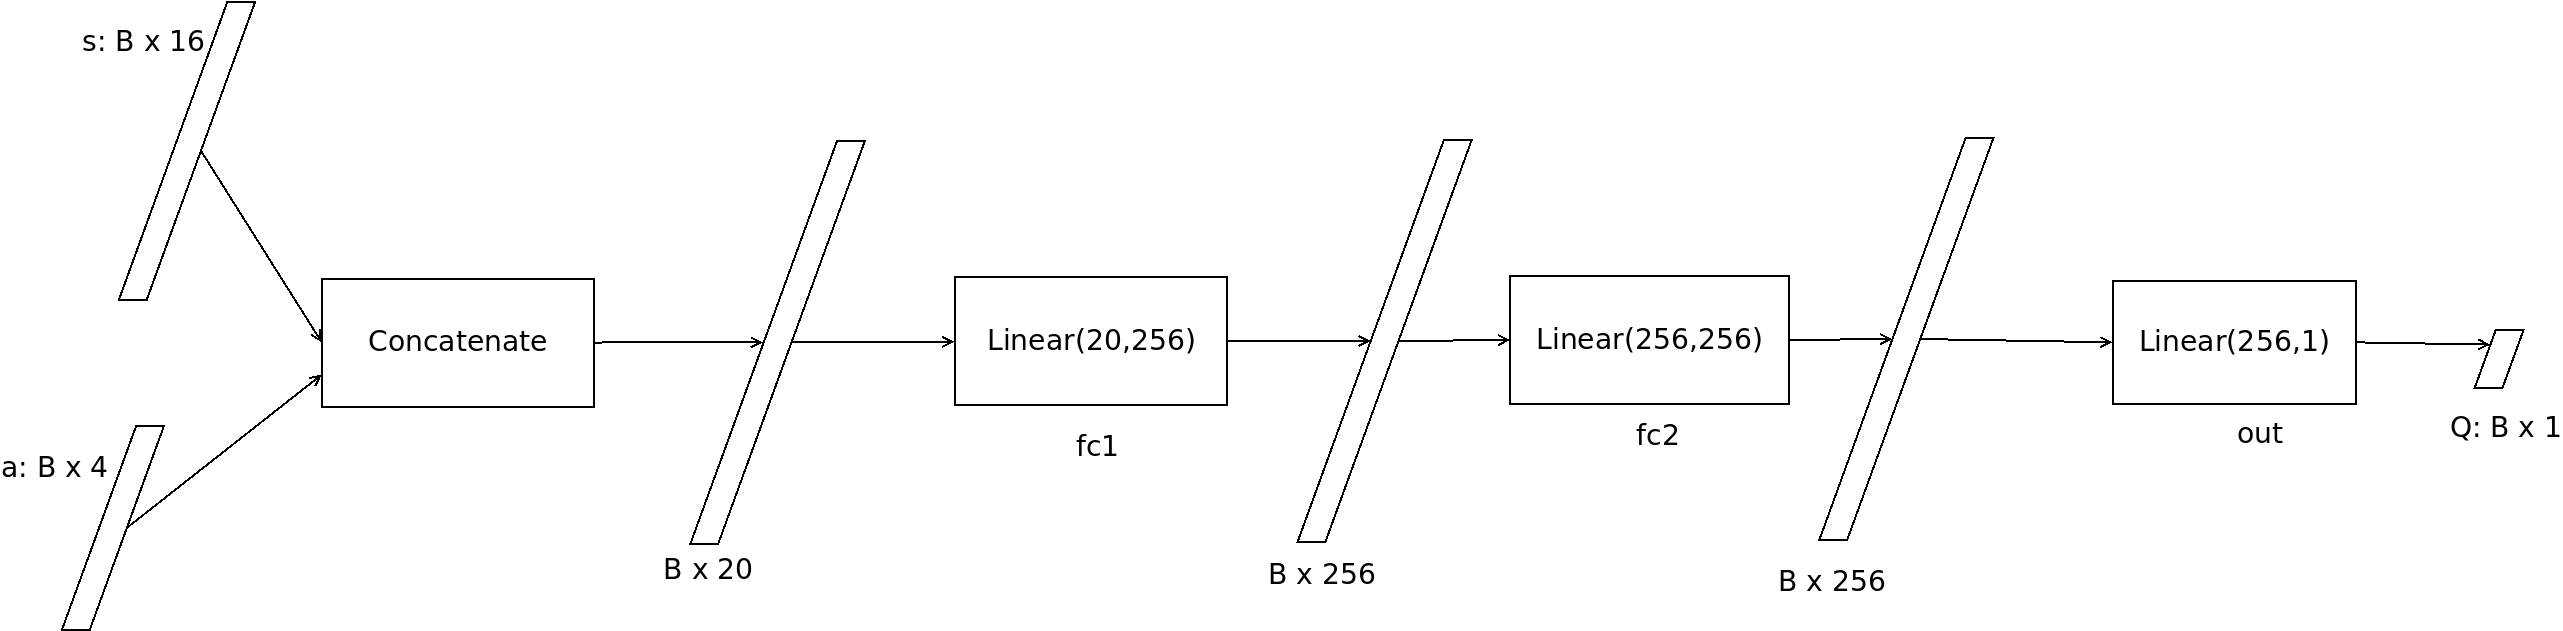
\includegraphics[width=\textwidth]{gymQnet.png}
        \caption{Gym环境下初步实验的评论家网络结构}
        \label{gymQnet}
    \end{figure}

上述$\mu$网络和$\mu$\_tar网络具有相同的网络结构,其网络结构如图\ref{gymMunet}所示。
    \begin{figure}
        \centering
        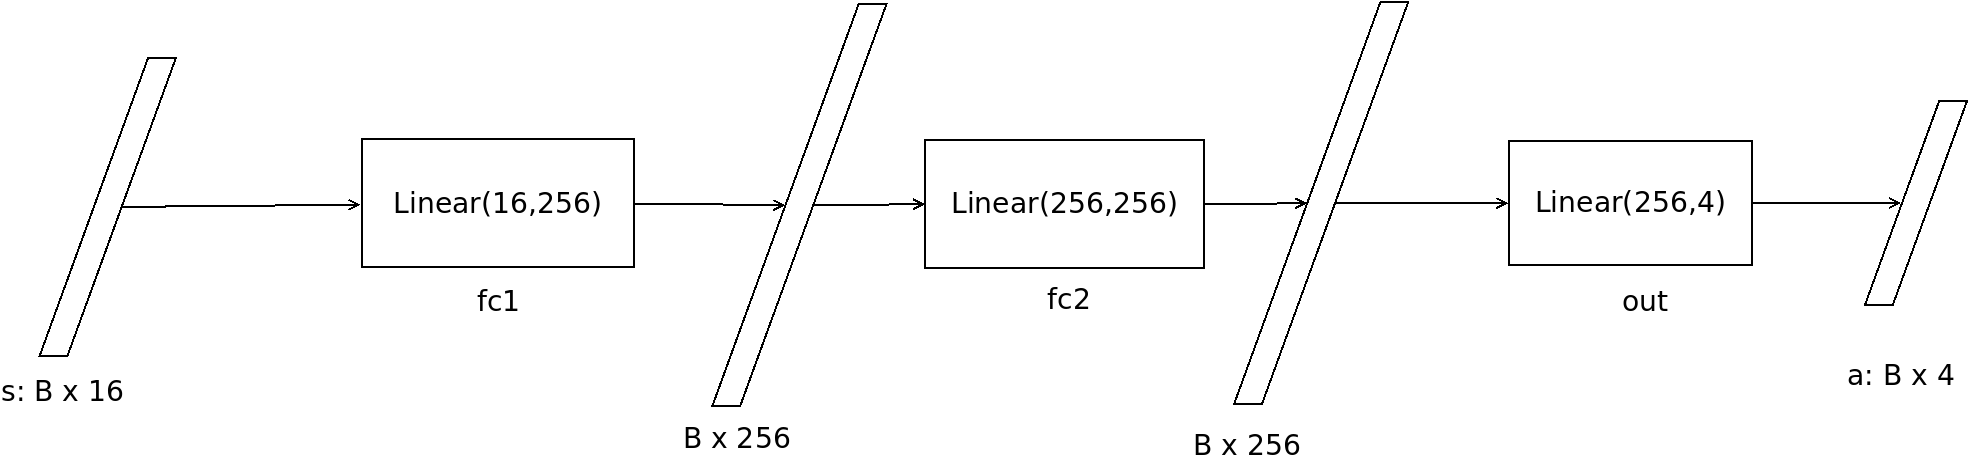
\includegraphics[width=\textwidth]{gymMunet.png}
        \caption{Gym环境下初步实验的演员网络结构}
        \label{gymMunet}
    \end{figure}

\section{Pyrobolearn主体实验系统设计}\label{myenvexp}
在Pyrobolearn框架中自定义的环境中有3种不同类型的状态构成了最终的状态向量:零件(link)世界速度状态、零件世界位置状态和物体位置状态。
在Pyrobolearn中,世界中的对象和机器人都被叫做物体(body)。
每个物体都有一个唯一的物体ID,它可以被世界对象用来找到对应的状态。
而机器人上面互相连接的构件被叫做零件(link)。
每个零件也有一个唯一的零件ID,它可被机器人对象用来找到对应的信息,而不能被世界对象直接访问。
零件的状态必须使用零件的ID来生成,使用物体ID生成零件状态或用零件ID生成物体状态都会导致严重的隐藏错误。

在实验中,WAM机械臂的末端执行器的ID可以使用get\_end\_effector\_ids来得到,而最后一个末端执行器的ID将在实验中用来生成已完成的目标向量$g^a$。
机器人上的一个零件的零件世界位置状态是一个3维的向量,而一个零件的零件世界速度状态是一个6维的向量。
如上所述,在实验中,直接把WAM机械臂的最后一个末端执行器的ID提供给了零件世界位置状态对象的构造方法,此状态对象可以用于监控已完成的目标向量$g^a$的值。
除了上述被选中的最后一个末端执行器,WAM机械臂还有20个其他零件。
每一个零件都有一个3维的世界位置状态和一个6维的世界速度状态。

实验中会有两个物体加载进\emph{Basic World}世界中,一个是上述WAM机械臂,另一个是一个初始位置随机的蓝色方块。
主体实验定义的开放任务为,WAM机械臂的最后一个末端执行器距离蓝色方块的距离应当在片段的最大时间步数限制内缩小到小于一个阈值,在每一个时间步,如果距离大于此阈值,则提供-1.0的奖励,否则提供0.0的奖励。
为了方便使用事后经验重放算法,需要在每个时间步获得蓝色方块的世界位置,用于监控这个期望目标向量$g^d$的状态可以很容易地使用方块的物体ID和物体世界位置构造方法来得到。

上文已经介绍了构成状态向量$s=(o, g^a, g^d)$中的已完成的目标$g^a$和期望目标$g^d$的定义,余下的$o$定义为WAM机械臂上的除了最后一个末端执行器的其他零件的世界位置和世界速度。
最终,这些状态构成了一个192维的状态向量$s\in \mathbb R^{192}$。
主体实验中使用到的这些状态并不是所有的状态。
根据通用机器人描述格式(Universal Robotic Description Format)中描述的模型,还有其他的状态(如图像传感器状态)可以被添加,但是现有的状态信息已经足够多以使得机械臂能够完成此开放任务,因此实验中没有添加更多状态。

在主体实验中,只使用了关节位置变化类型的动作作为机械臂与环境交互的动作。
在机械臂做出一个关节位置变化动作之后,关节的位置与动作值相加即可得到新的关节位置。
关节位置动作是一个15维的向量,这与\emph{FetchReach-v1}环境中的动作维度要高得多,因此在Pyrobolearn中自定义的此开放任务要比前者更难。

所有的实验中用到的动作和状态都是连续的,当考虑到状态空间和动作空间都是连续的这一事实后,可以知道智能体要搜索的空间是非常巨大的,这与上文定义的稀疏奖励结合起来就引出了在此开放任务下探索策略的问题。
在接下来的实验中,多个探索策略被提出以获得更高效率的探索,并更好地解决此问题。

Pyrobolearn下的实验程序的类图如图\ref{myenvuml}所示。
    \begin{figure}
        \centering
        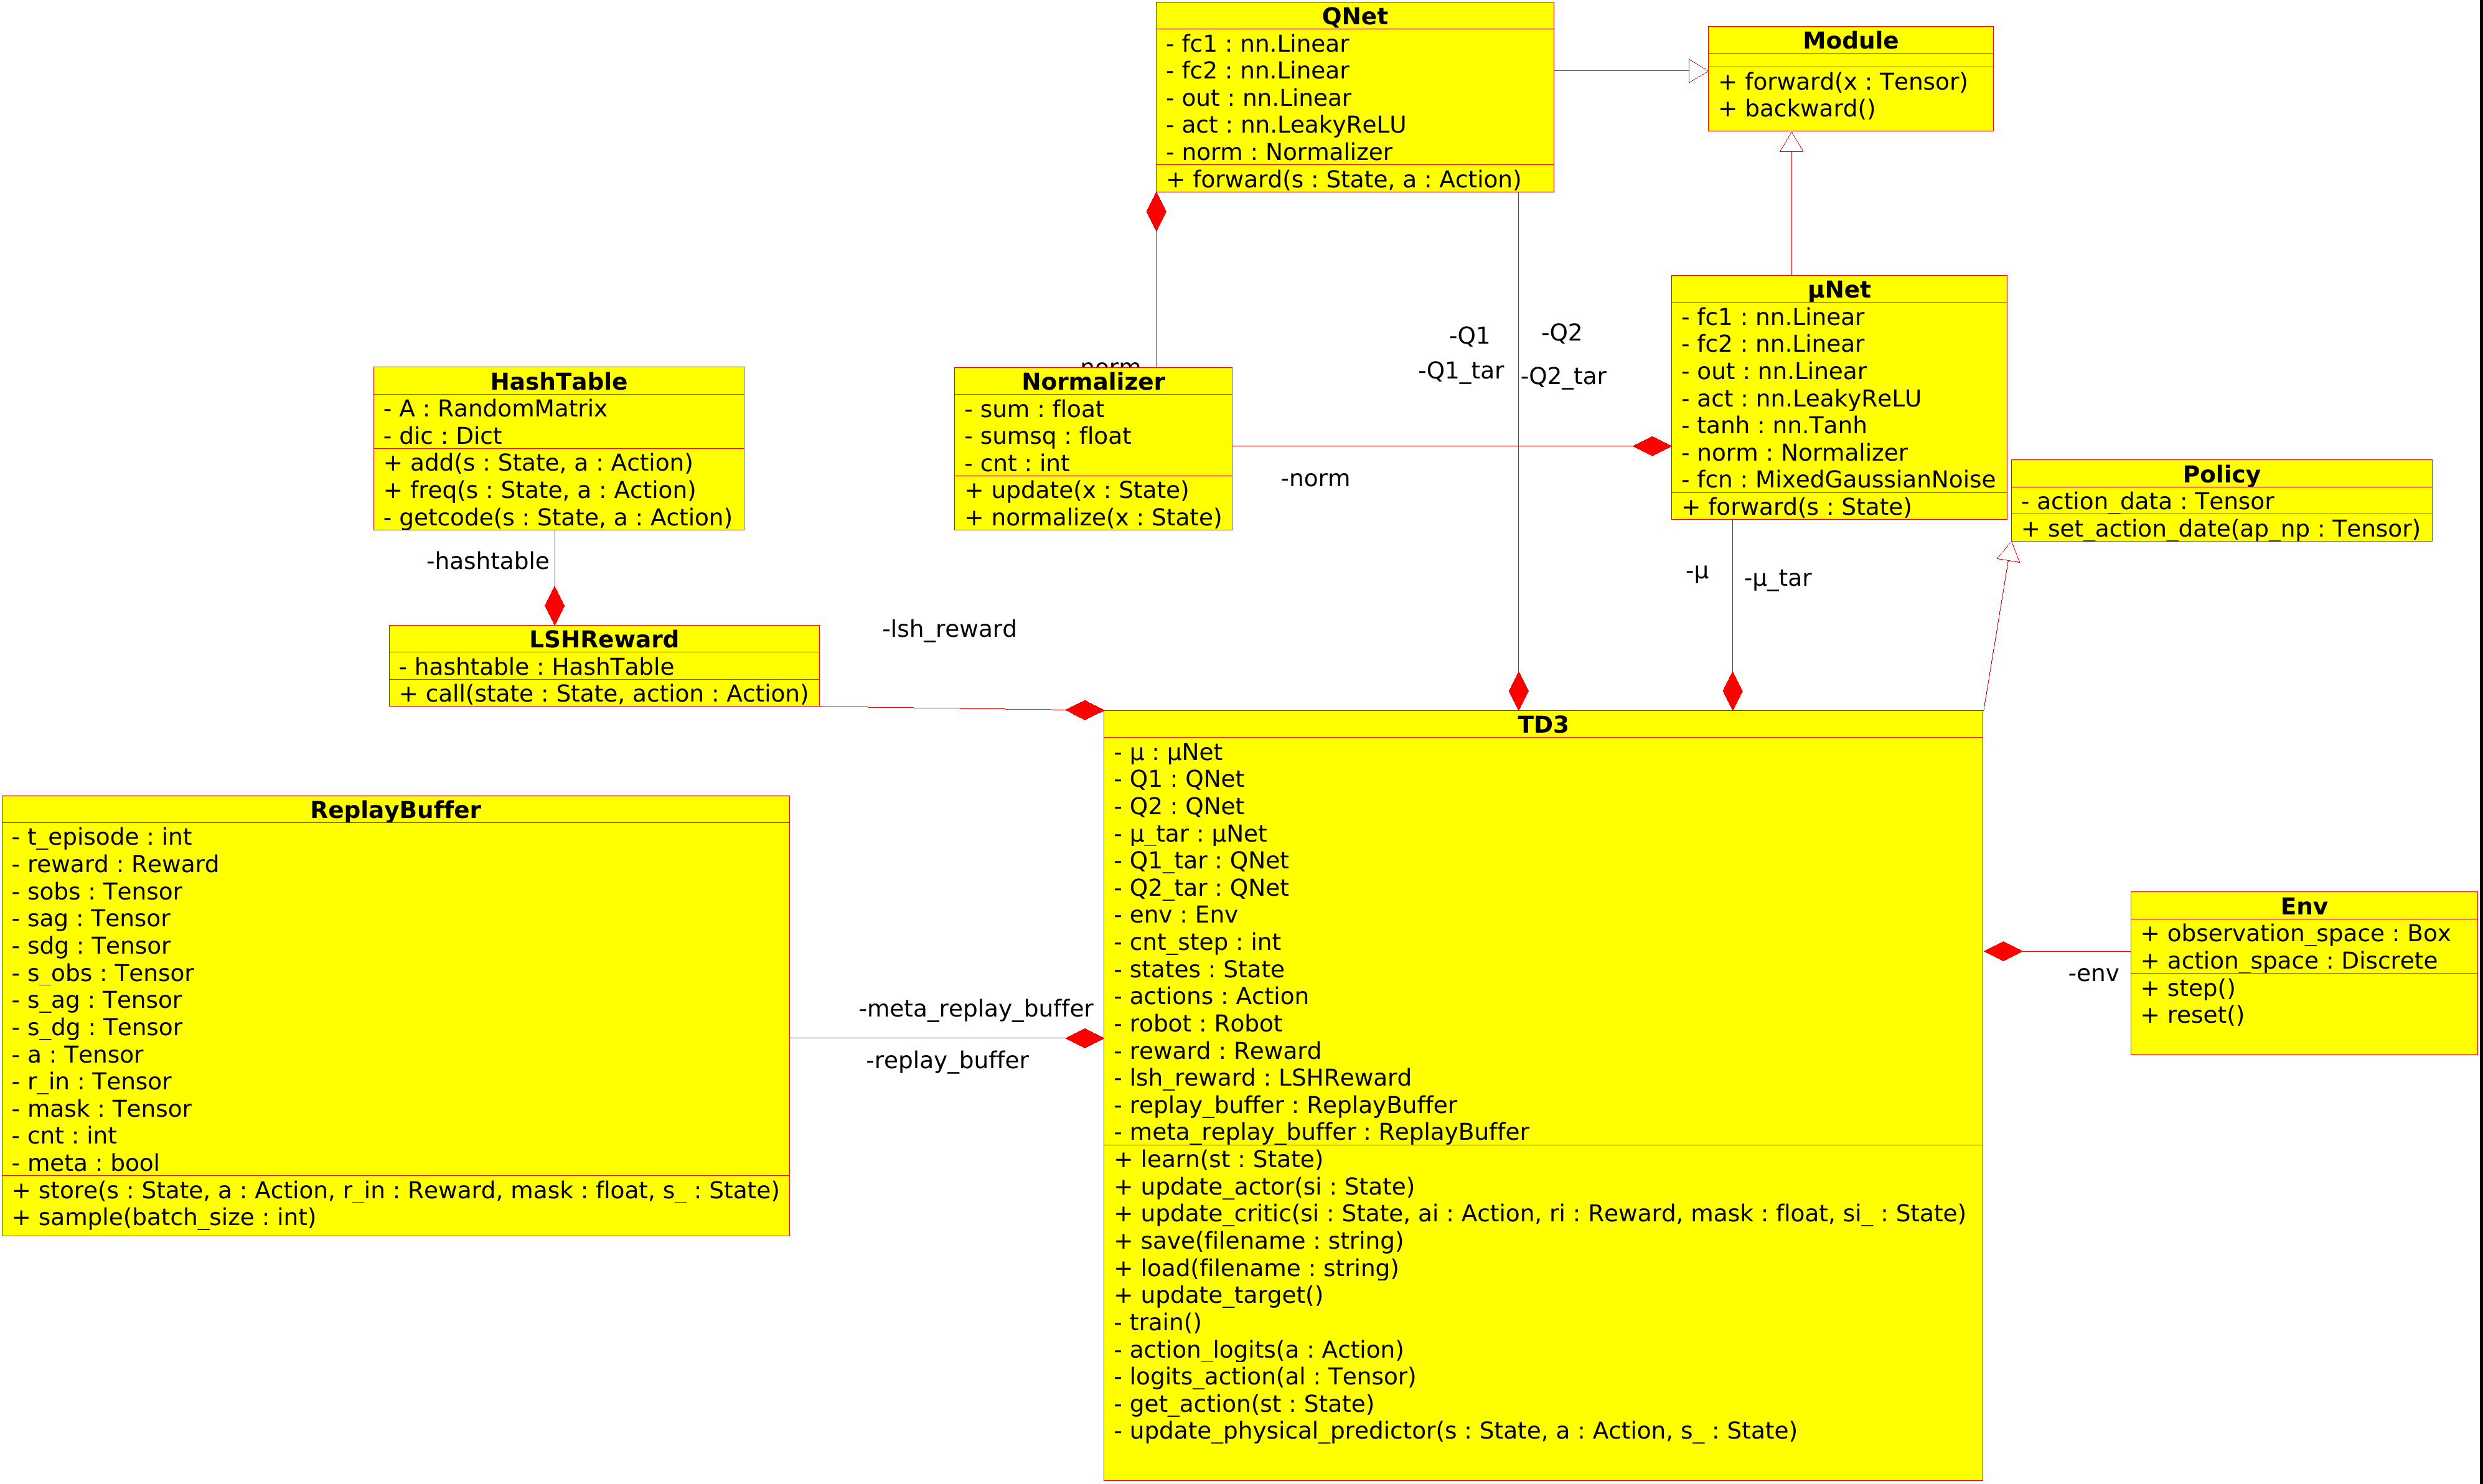
\includegraphics[width=\textwidth]{myenvuml.png}
        \caption{Pyrobolearn主体实验程序类图}
        \label{myenvuml}
    \end{figure}
    其与Gym环境中的初步实验程序的主要区别在于引入了基于局部敏感哈希的内部奖励函数对象LSHReward,正态化器Normalizer,Leaky ReLU激活层,高斯噪声层MixedGaussianNoise和元重放缓冲meta\_replay\_buffer的引入。
    元重放缓冲用于在$t<T_{start}$的时间内,未提供环境奖励时,保存内部奖励对应的迁移。
    另外在其中一个主体实验中还使用了update\_physical\_predictor方法来对正向动力学预测模型进行更新和训练,其中此模型的损失被用于构成内部奖励。
    为了方便演员网络使用Tanh激活层输出,策略TD3中还引入了action\_logits来把动作向量的每个元素的值都缩放到[-1,1],并使用logits\_action来进行反向解码出动作。

    与初步实验中类似,主体实验也使用全连接网络,但在演员网络中最后一层加入了混合高斯噪声层并与原网络输出动作求和,并且对输入层输出层进行了相应调整以适应输入数据。
    由于输入输出主体实验中所有神经网络的动作向量都进行了缩放,演员网络的最后一层不需要再乘以max\_action,只需要直接输出[-1,1]的缩放后的动作值,在策略TD3中调用演员网络的地方会自动进行缩放。

    主体实验中使用的演员网络结构如图\ref{myenvMunet}所示。
    主体实验中使用的评论家网络结构如图\ref{myenvQnet}所示。
    \begin{figure}
        \centering
        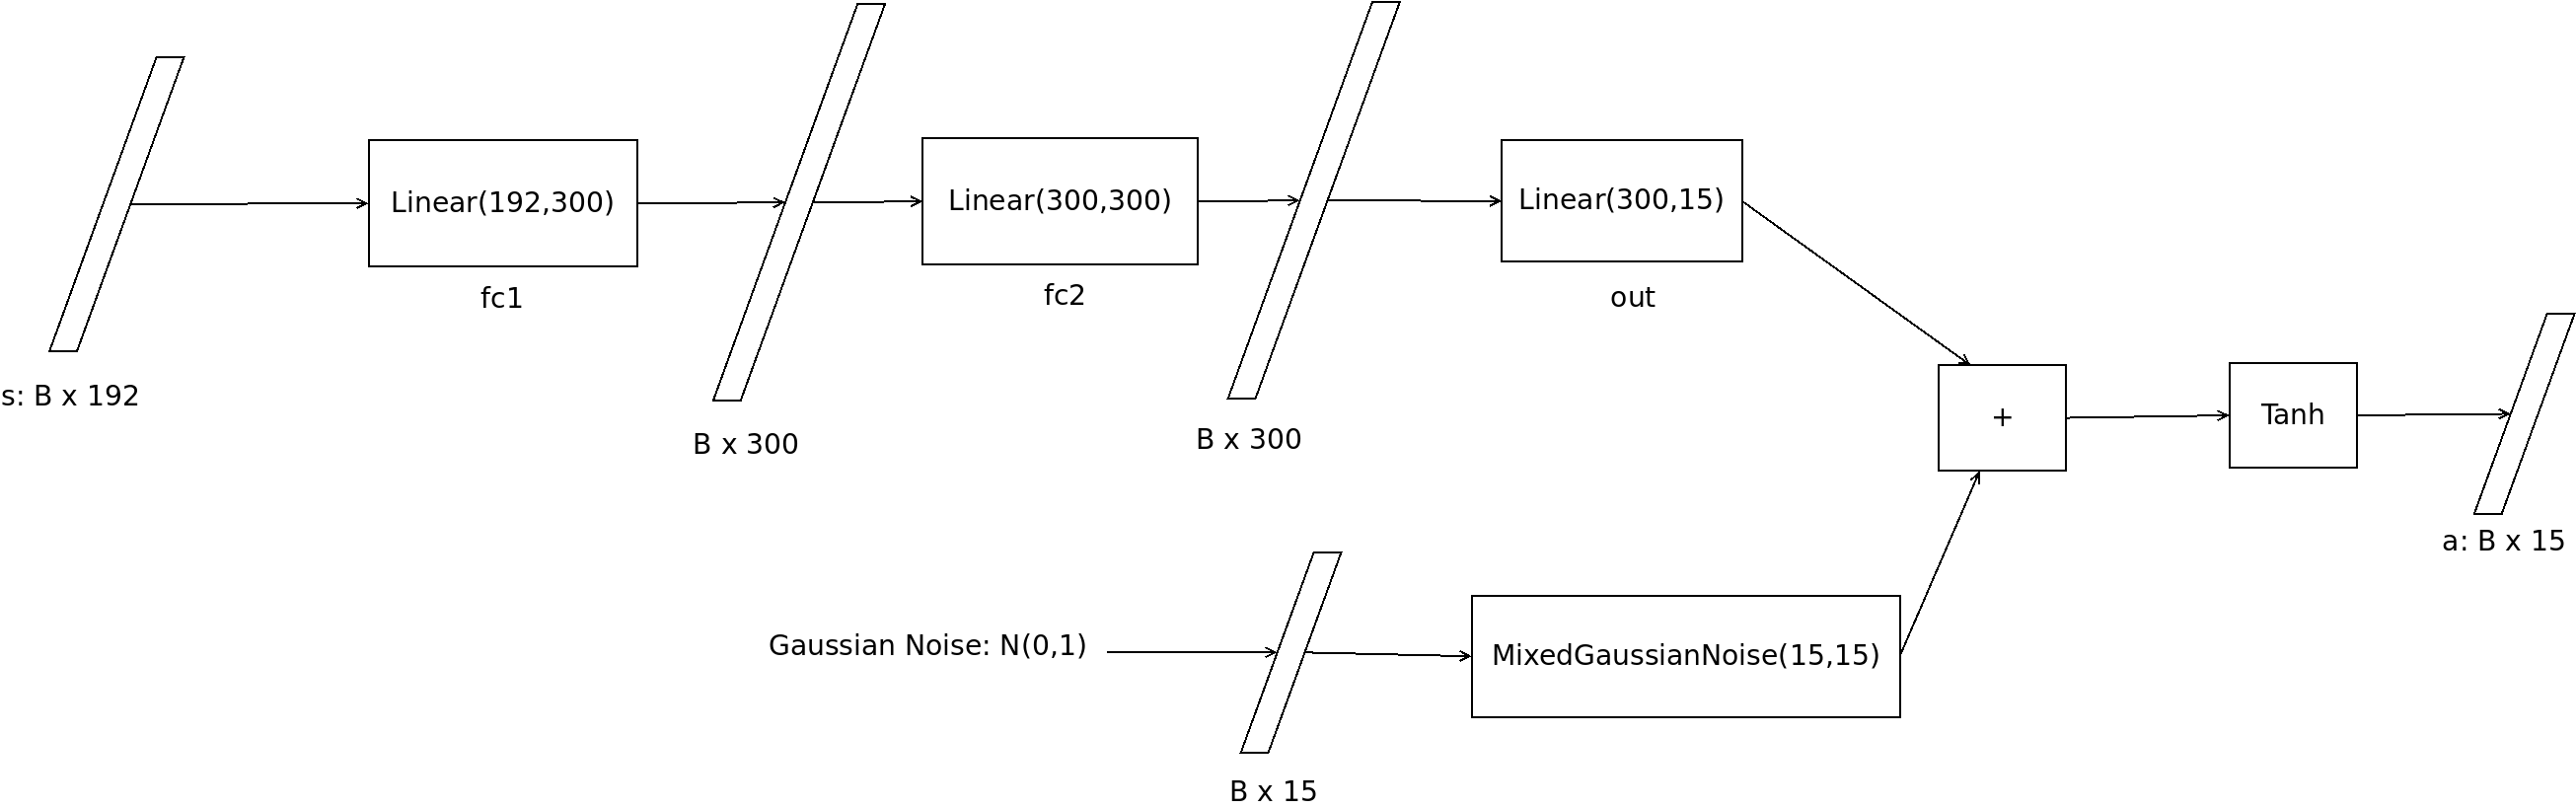
\includegraphics[width=\textwidth]{myenvMunet.png}
        \caption{Pyrobolearn中主体实验演员网络结构}
        \label{myenvMunet}
    \end{figure}

    \begin{figure}
        \centering
        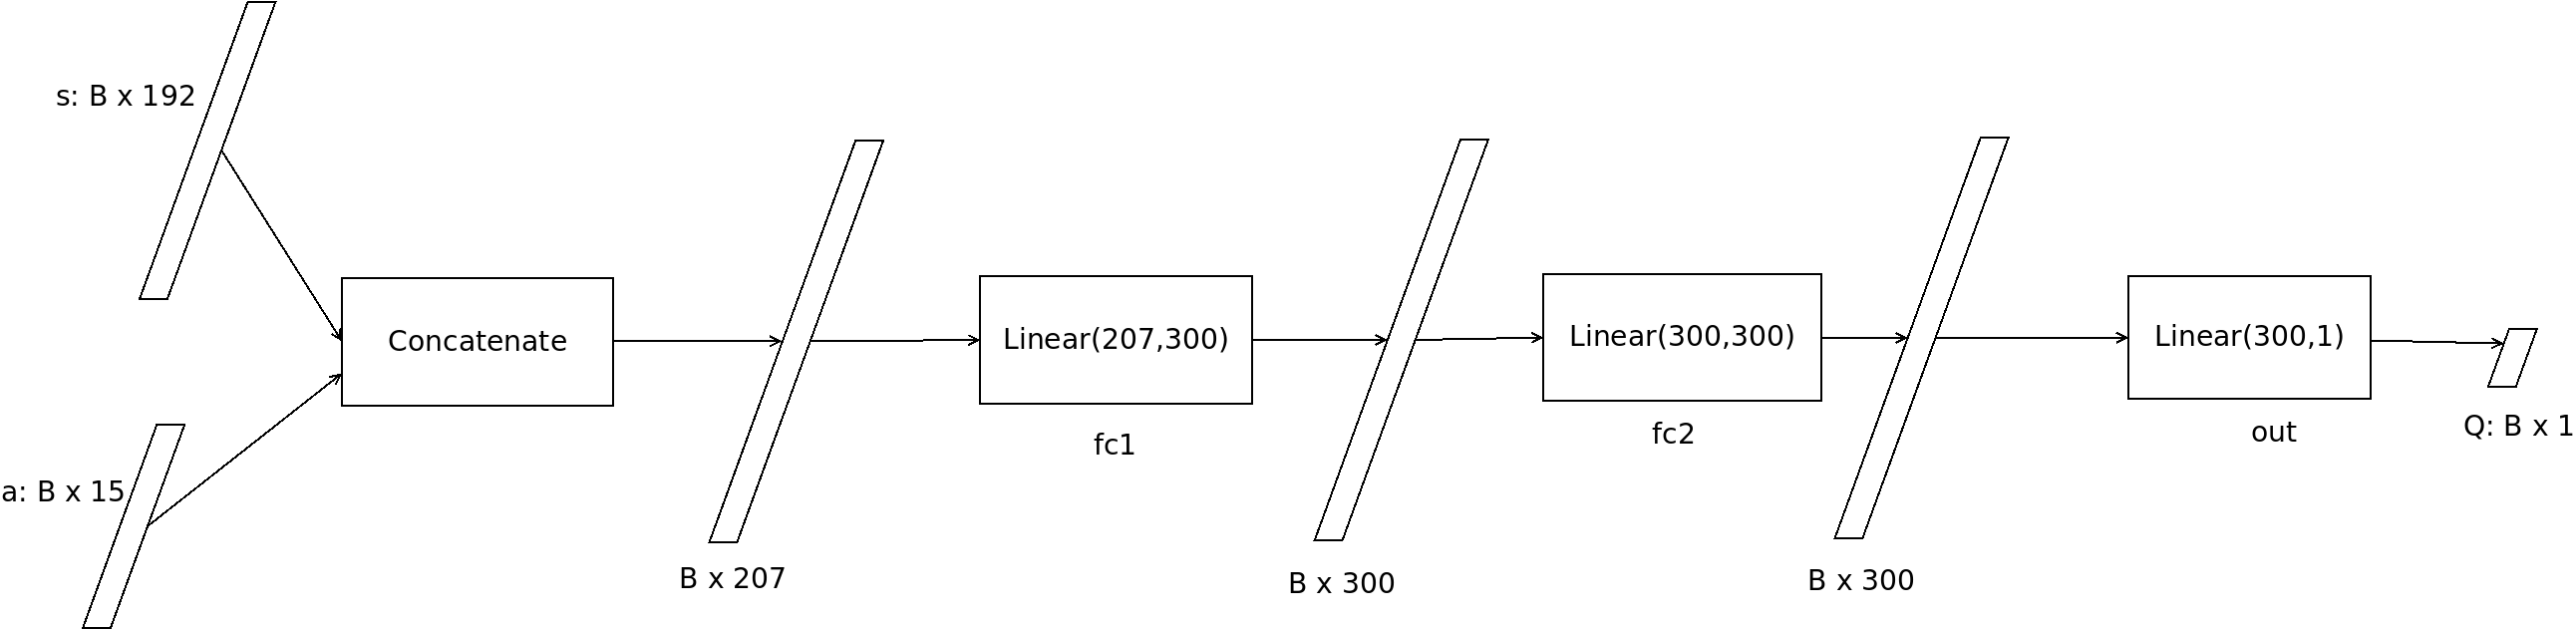
\includegraphics[width=\textwidth]{myenvQnet.png}
        \caption{Pyrobolearn中主体实验评论家网络结构}
        \label{myenvQnet}
    \end{figure}
% Local Variables:
% TeX-master: "../main"
% TeX-engine: xetex
% End:
